% !TeX spellcheck = pt_PT
\documentclass[11pt,a4paper]{article}
\usepackage[utf8]{inputenc}
\usepackage{etex}
\reserveinserts{28}



\usepackage{hyperref}
\usepackage{amsthm}
\usepackage{amsmath}
\usepackage{amssymb}
\usepackage{amsfonts}

\usepackage{pictex}
\usepackage[dvips]{graphics}
\usepackage{enumerate}

\usepackage{amsmath}
\usepackage{amssymb}
\usepackage{amsfonts}
\usepackage[portuguese]{babel}
\usepackage{pictex}
\usepackage[dvips]{graphics}
\usepackage{enumerate}
\usepackage{indentfirst}
\usepackage{listings}
\usepackage{tabularx}
\usepackage{multirow}
\usepackage{float}
\usepackage{makeidx}


\usepackage[usenames,dvipsnames]{color}

\usepackage{listings}

\definecolor{mygreen}{rgb}{0,0.6,0}
\definecolor{mygray}{rgb}{0.5,0.5,0.5}
\definecolor{mymauve}{rgb}{0.58,0,0.82}

\usepackage{graphicx}
\setlength{\parindent}{1cm}
\title{\bf{Compiladores - Projecto}\vspace{50mm}\\iJava\vspace{80mm}}
\author{
\textbf{Login Mooshak: TeamTransformadaZ}\\
João Ricardo Lourenço, Nº 2011151194\\
Joaquim Pedro Bento Gonçalves Pratas Leitão, Nº 2011150072}
\makeindex
\lstset{ %
  backgroundcolor=\color{white},   % choose the background color; you must add \usepackage{color} or \usepackage{xcolor}
  basicstyle=\footnotesize,        % the size of the fonts that are used for the code
  breakatwhitespace=false,         % sets if automatic breaks should only happen at whitespace
  breaklines=true,                 % sets automatic line breaking
  captionpos=b,                    % sets the caption-position to bottom
  commentstyle=\color{mygreen},    % comment style
  deletekeywords={...},            % if you want to delete keywords from the given language
  escapeinside={\%*}{*)},          % if you want to add LaTeX within your code
  extendedchars=true,              % lets you use non-ASCII characters; for 8-bits encodings only, does not work with UTF-8
  frame=single,                    % adds a frame around the code
  keepspaces=true,                 % keeps spaces in text, useful for keeping indentation of code (possibly needs columns=flexible)
  keywordstyle=\color{blue},       % keyword style
  language=C,                 % the language of the code
  morekeywords={*,...},            % if you want to add more keywords to the set
  numbers=left,                    % where to put the line-numbers; possible values are (none, left, right)
  numbersep=5pt,                   % how far the line-numbers are from the code
  numberstyle=\tiny\color{mygray}, % the style that is used for the line-numbers
  rulecolor=\color{black},         % if not set, the frame-color may be changed on line-breaks within not-black text (e.g. comments (green here))
  showspaces=false,                % show spaces everywhere adding particular underscores; it overrides 'showstringspaces'
  showstringspaces=false,          % underline spaces within strings only
  showtabs=false,                  % show tabs within strings adding particular underscores
  stepnumber=1,                    % the step between two line-numbers. If it's 1, each line will be numbered
  stringstyle=\color{mymauve},     % string literal style
  tabsize=2,                       % sets default tabsize to 2 spaces
  title=\lstname                   % show the filename of files included with \lstinputlisting; also try caption instead of title
}
\begin{document}

\maketitle
\centerline{\textbf{Relatório}}
\pagebreak

\printindex

\renewcommand*\contentsname{Índice}
\tableofcontents

\pagebreak


\section{Introdução}

No presente trabalho pretende-se desenvolver um compilador para a linguagem $iJava$, um pequeno subconjunto da linguagem Java (versão 5.0). Por ser um subconjunto de uma outra linguagem, todos os programas que respeitem as regras impostas em $iJava$ são também, garantidamente, programas válidos em $Java$\footnote{No entanto, certas restrições semânticas tornam certos códigos compiláveis e executáveis em iJava, mas não em Java. Um exemplo é o de código não acessível, que não é aceite pelo compilador javac, mas é válido em iJava.}.

Nesta linguagem todos os programas são constituídos por uma única classe, que possui métodos e atributos estáticos e públicos. Para além disso, a classe necessita obrigatoriamente de ter um método $main$, onde a execução do programa se inicia, com a mesma sintaxe do método main do Java. 

Podemos utilizar literais dos tipos inteiro e booleano e variáveis inteiras, booleanas e arrays uni-dimensionais de inteiros e booleanos.

A linguagem implementa também expressões aritméticas e lógicas, operações relacionais simples, e instruções de atribuição e controlo ($if-else$ e $while$).

Os métodos definidos, e os respetivos valores de retorno, podem ser de qualquer tipo acima mencionado, com exceção do método $main$, que, tal como em $Java$, possui como tipo de retorno o tipo $void$.

É também possível passar parâmetros (literais inteiros) ao nosso programa através da linha de comandos. É o método $main$ que vai receber esses parâmetros, armazenando-os num array de objetos do tipo $String$. No entanto, este tipo de dados não está incluído na lista de tipos permitidos em $iJava$, pois a sua utilização apenas é permitida no método $main$, com a mera finalidade de obter os parâmetros passados ao programa aquando da sua invocação. Deste modo, este array apenas suporta duas operações: o operador .length e a obtenção de um inteiro a partir dos seus elementos com $Integert.parseInt$.

O desenvolvimento do compilador foi dividido em três fases distintas.

Numa primeira fase foi realizada a \emph{Análise Lexical} do programa fonte, onde são identificados \emph{tokens}, isto é, cadeias pertencentes à linguagem e que têm significado e relevância para o programa.

Seguiram-se a realização da \emph{Análise Sintática} e \emph{Análise Semântica}, compostas por quatro etapas principais:

\begin{itemize}
\item \textbf{Tradução da gramática-fonte} (fornecida em notação $EBNF$) para o yacc e realização da \textbf{Análise Sintática} do programa, permitindo assim reconhecer se as sequências de \emph{tokens} que o constituem pertencem à linguagem, permitindo-nos assim detetar eventuais erros de sintaxe.

\item \textbf{Construção da árvore de sintaxe abstrata}, etapa realizada em simultâneo com a \textbf{Análise Sintática}. A árvore de sintaxe abstrata irá representar o nosso programa a compilar, recorrendo a uma estrutura em árvore para representar as estruturas sintáticas das cadeias que o constituem.

\item \textbf{Construção das tabelas de símbolos}, utilizadas para armazenar informações relevantes sobre a classe (seus atributos e métodos), bem como sobre cada método definido pelo programador (mais concretamente o tipo de retorno e os argumentos).

\item \textbf{Verificação de erros semânticos}, etapa principal da \textbf{Análise} \\* \textbf{Semântica}, onde são realizadas verificações de tipos, garantindo que para cada operação a realizar não existem incompatibilidades de tipos entre os operandos nela envolvidos.

\end{itemize}

A última fase do trabalho consistiu na \emph{Geração de Código Intermédio}, da qual resulta, na representação intermédia de \emph{LLVM}, um programa equivalente ao que pretendemos compilar.

\pagebreak

\section{Análise Lexical}

Tal como referimos anteriormente, na \emph{Análise Lexical} procedemos à identificação dos \emph{tokens} da nossa linguagem. Para isso utilizámos a ferramenta $lex$, responsável por gerar analisadores lexicais para linguagens.

Assim, no nosso analisador, sempre que é detectada a presença de um comentário no programa a compilar, seja do tipo $// ...$ (comentários de apenas uma linha) ou do tipo $/* ... */$ (comentários multi-linha), os caracteres incluídos nesse comentário são ignorados.

Sempre que é detectado um carácter ou uma sequência de caracteres que não constitui nenhum \emph{token}, é detectado um erro lexical, sendo impressa uma mensagem de erro, indicando a existência de um caracter ilegal, juntamente com a sua posição no programa.

Adicionalmente, caso se verifique a ocorrência de um comentário multi-linha que não foi devidamente terminado, o erro lexical é também detectado, sendo impressa uma mensagem de erro que indica a posição no programa onde o comentário foi iniciado.

	\subsection{Tokens}

	Em seguida, apresentamos a lista dos \emph{tokens} válidos na linguagem $iJava$ e a lista dos \emph{tokens} reservados que, por essa razão, não estão disponíveis na nossa linguagem:
	
	\begin{itemize}
	\item \textbf{ID}: Sequências alfanuméricas (maiúsculas e minúsculas) começadas por uma letra, podendo conter também símbolos como $``\_''$ e $``\$''$. Este \emph{token} pode também ser descrito na forma da sua expressão regular: \emph{{letra}({letra}|{[0-9]})*}, sendo o \emph{token} \textbf{letra} da nossa autoria definido por: $[a-z] \mid [A-Z] \mid ``\_''|``\$''$
	
	\item \textbf{INTLIT}: Sequências de dígitos decimais e hexadecimais (incluindo a-f e A-F) precedidas de $0x$. Este \emph{token} pode também ser descrito na forma da seguinte expressão regular: \emph{{[0-9]}+|0x[0-9a-fA-F]+}
	
	\item \textbf{BOOLLIT}: $true \mid false$
	
	\item \textbf{INT}: $int$
	
	\item \textbf{BOOL}: $boolean$
	
	\item \textbf{NEW}: $new$
	
	\item \textbf{IF}: $if$
	
	\item \textbf{ELSE}: $else$
	
	\item \textbf{WHILE}: $while$
	
	\item \textbf{PRINT}: $System.out.println$
	
	\item \textbf{PARSEINT}: $Integer.parseInt$
	
	\item \textbf{CLASS}: $class$
	
	\item \textbf{PUBLIC}: $public$
	
	\item \textbf{STATIC}: $static$
	
	\item \textbf{VOID}: $void$
	
	\item \textbf{STRING}: $String$
	
	\item \textbf{DOTLENGTH}: $.length$
	
	\item \textbf{RETURN}: $return$
	
	\item \textbf{OCURV}: $($
	
	\item \textbf{CCURV}: $)$
	
	\item \textbf{OBRACE}: $\{$
	
	\item \textbf{CBRACE}: $\}$
	
	\item \textbf{OSQUARE}: $[$
	
	\item \textbf{CSQUARE}: $]$
	
	\item \textbf{OP1}: $\&\& \mid \mid \mid$
	
	\item \textbf{OP2}: $< \mid > \mid == \mid != \mid <= \mid >=$
	
	\item \textbf{OP3}: $"+" \mid ``-''$
	
	\item \textbf{OP4}: $"*" \mid ``/'' \mid ``\%''$
	
	\item \textbf{NOT}: $``!''$
	
	\item \textbf{ASSIGN}: $``=''$
	
	\item \textbf{SEMIC}: $``;''$
	
	\item \textbf{COMMA}: $``,"$
	
	\item \textbf{RESERVED}: $abstract \mid continue \mid for \mid switch \mid assert \mid default \mid goto \mid package \mid synchronized \mid do \mid private \mid this \mid break \mid double \mid implements \mid protected \mid throw \mid byte \mid import \mid throws \mid case \mid enum \mid instanceof \mid transient \mid catch \mid extends \mid short \mid try \mid char \mid final \mid interface \mid finally \mid long \mid strictfp \mid volatile \mid const \mid float \mid native \mid super \mid null \mid ++ \mid --$
	\end{itemize}

	Para além dos \emph{tokens} apresentados, definimos outros \emph{tokens}, que passamos a especificar:
	
	\begin{itemize}
	\item \textbf{NEWLINE}: $Token$ correspondente ao caracter de mudança de linha, $\setminus n$
	
	\item \textbf{WHITESPACE}:$Token$ correspondente ao caracter de espaço em branco
	
	\item \textbf{OPEN\_COMMENT}:  $Token$ correspondente ao início de um comentário multi-linha, $/*$
	
	\item \textbf{CLOSE\_COMMENT}: $Token$ correspondente ao fecho de um comentário multi-linha, $*/$
	
	\item \textbf{SINGLE\_LINE\_COMMENT}: $Token$ utilizado para detetar a \\* ocorrência de um comentário de uma linha apenas
	\end{itemize}
	
	Quando implementámos a \emph{Análise Sintática}, para resolver problemas de ambiguidade da gramática e permitir uma correcta análise semântica e geração de código, foi necessário, entre outras acções que iremos abordar na próxima secção, separar os \emph{tokens} \textbf{OP1}, \textbf{OP2}, \textbf{OP3} e \textbf{OP4} nas diferentes sequências alfanuméricas que os constituíam. Assim, temos ainda os seguintes \emph{tokens}:
	
	\begin{itemize}
	\item \textbf{AND} ("\&\&") e \textbf{OR} ("$||$"), originados a partir do \emph{token} \textbf{OP1}
	
	\item \textbf{LE} (``<''), \textbf{GE} (``>''), \textbf{EQ} (``==''), \textbf{NEQ} (``!=''), \textbf{LEQ} (``<='') e \textbf{GEQ} (``>=''), originados a partir do \emph{token} \textbf{OP2}
	
	\item \textbf{PLUS} (``+'') e \textbf {MINUS} (``-''), originados a partir do \emph{token} \textbf{OP3}
	
	\item \textbf{MULT} (``*''), \textbf{DIV} (``/'') e \textbf{MOD} (``\%''), originados a partir do \emph{token} \textbf{OP4}
	\end{itemize}
	
	\subsection{Comentários}
	
	Para identificarmos a ocorrência de comentários nos programas a compilar recorremos aos \emph{tokens} \emph{OPEN\_COMMENT}, \emph{CLOSE\_COMMENT} e \\* \emph{SINGLE\_LINE\_COMMENT}.
	
	Quando detectamos o \emph{token OPEN\_COMMENT} é criado um novo estado no analisador lexdical, que indica a existência de um comentário multi-linha. A esse estamos demos o nome \emph{MULTI\_LINE\_COMMENT\_S}.
	
	Uma vez neste estado, todos os caracteres e \emph{tokens} identificados são ignorados, com exceção do \emph{token} de fecho do comentário multi-linha \\* (\emph{CLOSE\_COMMENT}) e do \emph{token} de fim do ficheiro, $<<EOF>>$, disponível na ferramenta utilizada para desenvolver o analisador (\emph{lex}). 
	
	Caso seja identificado o \emph{token CLOSE\_COMMENT}, o estado do analisador é reposto, passando este a ter o seu estado por defeito. A utilização desta técnica permite-nos terminar após o primeiro $*/$, como desejado.
	
	Por outro lado, se for detectado $<<EOF>>$ temos uma situação em que um comentário multi-linha não foi devidamente terminado, pelo que é gerado um erro lexical, terminando a execução do analisador e sendo o utilizador informado da ocorrência do erro e da localização no programa fornecido do comando que inicia o comentário.
	
	Se, por alguma razão, o \emph{token CLOSE\_COMMENT} for identificado quando o analisador não se encontra no estado \emph{MULTI\_LINE\_COMMENT\_S} é detectada também a ocorrência de um erro lexical, uma vez que na nossa linguagem não é possível a existência do token \emph{*/} sem que antes tenha sido colocado um \emph{/*}. Mais uma vez, assim que o erro lexical é detectado, o utilizador é informado com uma mensagem que indica a posição no programa onde se deu o erro, e o analisador termina a sua execução.
	
	Ao detectarmos o \emph{token SINGLE\_LINE\_COMMENT} vamos ignorar todos os caracteres e \emph{tokens} que se lhe seguirem, até que seja reconhecido o \emph{token} de mudança de linha (\emph{NEWLINE}). Desta forma estamos a descartar toda a restante linha do programa, após a ocorrência de $//$, tal como seria desejado no tratamento de comentários de uma linha apenas.
	
	\subsection{Tratamento de Erros Lexicais}
	
	Tal como referimos nos pontos anteriores, sempre que o analisador desenvolvido detecta a ocorrência de um erro lexical (seja por existência de um \emph{token} não permitido ou por não término de um comentário multi-linha), é impressa uma mensagem de erro que indica a posição do erro no programa a compilar (indicando a linha e coluna onde o erro ocorreu).
	
	Quando é detectado um caracter ilegal, o analisador imprime a mensagem de erro, prosseguindo a sua execução na linha seguinte do programa a compilar até ser lido todo o conteúdo do programa.
	
	Tendo sido detectada a ocorrência de um ou mais erros lexicais, após ler todo o programa, o analisador termina a sua execução, não sendo realizado mais nenhum passo da compilação.


\pagebreak

\section{Análise Sintática}

A Análise Lexical permite-nos identificar os \emph{tokens} da linguagem, isto é, os seus ``átomos''. No entanto, interessa-nos garantir que os \emph{tokens} identificados estejam organizados de acordo com a estrutura sintática da linguagem.

Para validar essa organização dos \emph{tokens} necessitamos de utilizar uma gramática, que nos indica como devem estar organizados sintaticamente os \emph{tokens} da linguagem. Para além disso, utilizámos a ferramenta \emph{YACC (Yet Another Compiler Compiler)}, um gerador de analisadores sintáticos.

Assim, utilizamos o analisador lexical (\emph{lex}) desenvolvido para reconhecer os \emph{tokens} da linguagem, que são transferidos para o \emph{yacc} onde, com base na gramática da linguagem fornecida, podemos verificar se o programa a compilar se encontra organizado de acordo com a estrutura sintática da linguagem.

No analisador sintático foi criada uma \emph{union}, que define a estrutura de uma variável \emph{yylval}, utilizada na comunicação entre o \emph{yacc} e o \emph{lex}. Apresentamos desde já a estrutura da \emph{union} criada:

\begin{lstlisting}
%union
{
    char* token;    
    struct _node_t* node;
    int type;
}
\end{lstlisting}

Os \emph{tokens} detectados no \emph{lex} são comunicados ao analisador sintático através do campo \emph{token} da variável \emph{yylval}.

Para além disso, no analisador sintático declaramos ainda três variáveis externas, para uso partilhado entre o \emph{lex} e o \emph{yacc}: Duas do tipo inteiro, \emph{prev\_col} e \emph{prev\_line}, e uma do tipo array de caracteres (\emph{char*}), chamada \emph{yytext} e que contém a cadeia de caracteres lida pelo analisador, em cada momento. Esta variável é implementada/definida internamente pelo \emph{lex}.

Tal como o nome pode sugerir, \emph{prev\_col} e \emph{prev\_line} são utilizadas para armazenar o valor da coluna e linha (do programa a compilar) analisadas na iteração anterior da execução do analisador. A justificação para esta escolha prende-se com as situações onde ocorrem erros sintáticos, sendo necessário informar o utilizador da localização no programa desse erro.

\begin{figure}[H]
  \centering
      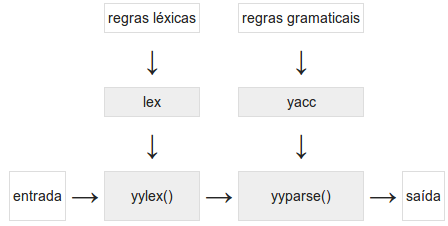
\includegraphics[scale=0.5]{DiagramaLExYACC.png}
  \caption{Ligação entre o \emph{lex} e o \emph{yacc}, ferramentas utilizadas para gerar os analisadores lexicais e sintáticos. Retirado de \emph{http://pt.wikipedia.org/wiki/Yacc}}
\end{figure}

\subsection{Gramática}

De seguida, apresentamos a gramática da linguagem \emph{iJava}, fornecida no enunciado do projeto, em notação \textbf{EBNF}:

\vspace{0.5cm}

\hspace{-1cm}Start $\rightarrow$ Program

\hspace{-1cm}Program $\rightarrow$ CLASS ID OBRACE \{ FieldDecl $\mid$ MethodDecl \} CBRACE

\hspace{-1cm}FieldDecl $\rightarrow$ STATIC VarDecl

\hspace{-1cm}MethodDecl $\rightarrow$ PUBLIC STATIC ( Type $\mid$ VOID ) ID OCURV

\hspace{-.5cm}[ FormalParams ] CCURV OBRACE \{ VarDecl \} \{ Statement \} CBRACE

\hspace{-1cm}FormalParams $\rightarrow$ Type ID \{ COMMA Type ID \}

\hspace{-1cm}FormalParams $\rightarrow$ STRING OSQUARE CSQUARE ID

\hspace{-1cm}VarDecl $\rightarrow$ Type ID \{ COMMA ID \} SEMIC

\hspace{-1cm}Type $\rightarrow$ ( INT $\mid$ BOOL ) [ OSQUARE CSQUARE ]

\hspace{-1cm}Statement $\rightarrow$ OBRACE \{ Statement \} CBRACE

\hspace{-1cm}Statement $\rightarrow$ IF OCURV Expr CCURV Statement [ ELSE Statement ]

\hspace{-1cm}Statement $\rightarrow$ WHILE OCURV Expr CCURV Statement

\hspace{-1cm}Statement $\rightarrow$ PRINT OCURV Expr CCURV SEMIC

\hspace{-1cm}Statement $\rightarrow$ ID [ OSQUARE Expr CSQUARE ] ASSIGN Expr SEMIC

\hspace{-1cm}Statement $\rightarrow$ RETURN [ Expr ] SEMIC

\hspace{-1cm}Expr $\rightarrow$ Expr ( OP1 $\mid$ OP2 $\mid$ OP3 $\mid$ OP4 ) Expr

\hspace{-1cm}Expr $\rightarrow$ Expr OSQUARE Expr CSQUARE

\hspace{-1cm}Expr $\rightarrow$ ID $\mid$ INTLIT $\mid$ BOOLLIT

\hspace{-1cm}Expr $\rightarrow$ NEW ( INT $\mid$ BOOL ) OSQUARE Expr CSQUARE

\hspace{-1cm}Expr $\rightarrow$ OCURV Expr CCURV

\hspace{-1cm}Expr $\rightarrow$ Expr DOTLENGTH $\mid$ ( OP3 $\mid$ NOT ) Expr

\hspace{-1cm}Expr $\rightarrow$ PARSEINT OCURV ID OSQUARE Expr CSQUARE CCURV

\hspace{-1cm}Expr $\rightarrow$ ID OCURV [ Args ] CCURV

\hspace{-1cm}Args $\rightarrow$ Expr \{ COMMA Expr \}

\vspace{0.5cm}

Lembramos que, em notação \textbf{ENBF}, os símbolos \textbf{[...]} englobam \emph{tokens} opcionais e \textbf{\{...\}} implicam a repetição dos \emph{tokens} 0 ou mais vezes.

\subsubsection{Ambiguidade}

Um análise mais cuidada da gramática apresentada permite-nos aferir da sua ambiguidade. Por exemplo, se num dado momento da análise sintática pretendermos analisar $2+3*5$, podemos reduzir esta expressão à variável \emph{EXPR} da gramática por duas formas distintas:

\begin{enumerate}
\item Numa primeira abordagem podemos separar a expressão em \textbf{Expr $\rightarrow$ Expr + Expr} (onde o símbolo \emph{"+"} é proveniente do \emph{token} \emph{OP3}). De seguida reduziríamos o primeiro símbolo \emph{Expr} para o \emph{token} \emph{INTLIT} correspondente, neste caso, ao literal \emph{"2"}. O segundo símbolo \emph{Expr} seria desdobrado em \textbf{Expr $\rightarrow$ Expr * Expr} (onde o símbolo \emph{"*"} é proveniente do \emph{token} \emph{OP4}). Neste caso os dois símbolos \emph{Expr} seriam reduzidos ao \emph{token} \emph{INTLIT}, correspondente a cada um dos restantes literais.

\item Numa abordagem alternativa começaríamos por separar a expressão em \textbf{Expr $\rightarrow$ Expr * Expr}. De seguida desdobraríamos o primeiro símbolo \emph{Expr} em \textbf{Expr $\rightarrow$ Expr + Expr}. Estes dois novos símbolos \emph{Expr} seriam reduzidos a \emph{INTLIT}, tal como o restante símbolo \emph{Expr}.
\end{enumerate}

Acabámos de provar a ambiguidade da gramática. Tal como esta situação existem muitas outras envolvendo os operadores englobados pelos \emph{tokens} \emph{OP1, OP2, OP3 e OP4}. Assim, é imperativa a definição de prioridades nos operadores, de forma a eliminar todas as ambiguidades presentes na gramática, permitindo assim a correta realização da análise sintática do programa. A definição de prioridades também nos auxiliará a definir concisamente as prioridades que o Java implementa.

\subsection{Alterações à Gramática Fornecida}

Uma vez que a gramática apresentada é ambígua e está apresentada em notação \textbf{EBNF}, não aceite pela ferramenta utilizada para gerar o analisador sintático, necessitámos de alterar a gramática, de forma a eliminar as suas ambiguidades, tornando-a numa gramática aceite pela ferramenta utilizada.

\subsubsection{Definição de Novos \emph{Tokens}}

Como já referimos, a primeira alteração realizada prende-se com a separação dos operadores englobados pelos \emph{tokens} \emph{OP1, OP2, OP3 e OP4}, criando um novo \emph{token} para cada operador, definindo de seguida a prioridade dos diferentes operadores representados pelos \emph{tokens} criados.

As prioridades dos operadores foram definidas na ferramenta \emph{yacc}, de acordo com a sua notação. De seguida apresentamos a definição, em notação \emph{yacc} da prioridade dos operadores identificados:

\begin{lstlisting}
%nonassoc THEN
%nonassoc ELSE
%nonassoc REDUCEEXPRESSON1
%left OR
%left AND
%left EQ NEQ
%left LE GE LEQ GEQ
%left PLUS MINUS
%left MULT DIV MOD
%right ASSIGN
%left OBRACE
%right UNARY_HIGHEST_VAL
%left OSQUARE DOTLENGTH
\end{lstlisting}

\vspace{0.5cm}

Na notação \emph{yacc} a prioridade de um \emph{token} é definida com as instruções \emph{\%left} e \emph{\%right}, correspondendo respetivamente à associatividade à esquerda ou à direita. Alternativamente podemos também utilizar a instrução \emph{\%nonassoc}, indicando que o operador não tem qualquer associatividade. Para além disso a prioridade de um operador é tanto maior quanto posterior for a sua definição.

Na situação apresentada indicamos, por exemplo, que os operadores \emph{THEN} e \emph{ELSE} não têm qualquer associatividade, tendo o operador \emph{ELSE} maior prioridade do que o operador \emph{THEN}.

Chamamos a atenção para os \emph{tokens} \emph{REDUCEEXPRESSION1}, \\* \emph{THEN}, \emph{ELSE}, e\emph{UNARY\_HIGHEST\_VAL}, que passamos a detalhar mais à frente.

\subsubsection{Indexação de Expressões}

À semelhança do que acontece em \emph{Java}, também em \emph{iJava} existem expressões passíveis de serem indexadas e outras onde a operação de indexação não é possível. A nível sintáctico, optámos por estruturar a detecção destes erros de acordo com o seguinte catálogo:

\begin{itemize}
\item \textbf{Expressões Não-Indexáveis:} Declarações de arrays (inteiros e booleanos), expressões compostas apenas por símbolos terminais (literais inteiros ou booleanos) e expressões onde já é realizada indexação (ou seja, indexáveis)

\item \textbf{Expressões Indexáveis:} Todas as restantes
\end{itemize}

Realçamos que nem todas as restantes expressões são indexáveis, mas que a verificação da correcta indexação destas é delegada para a análise semântica.

\subsubsection{Expressões Não-Indexáveis}

Dadas as características da linguagem descritas em secções anteriores, uma vez que em \emph{iJava} apenas está disponível a utilização de arrays uni-dimensionais, não podemos considerar as declarações de arrays indexáveis. Caso o fizéssemos, a operação \emph{new int[5][2]} seria válida na nossa linguagem.

De facto, poderíamos entender esta instrução como a declaração de um array uni-dimensional de inteiros, e o posterior acesso à sua terceira posição. No entanto, esta operação corresponde, na linguagem \emph{Java} à declaração de um array bi-dimensional de inteiros, não permitido em \emph{iJava}.

Assim, consideramos a operação \emph{new int[5][2]} inválida na linguagem \emph{iJava}, o que nos permite concluir que todas as declarações de arrays não são indexáveis. Para além disso, caso um programador pretenda declarar um array uni-dimensional e aceder de seguida a uma das suas posições, na mesma linha de código, também o poderá fazer em \emph{iJava}, devendo envolver a declaração do array numa expressão indexável, através da utilização de parêntesis: emph{(new int[5])[2]}.

\subsubsection{Expressões Indexáveis}

Todas as expressões que não declarações de arrays ou terminais são passíveis de serem indexadas na nossa linguagem.

Queremos, contudo, chamar a atenção para situações não permitidas na linguagem, como por exemplo \emph{a[0]} caso \emph{a} seja uma variável do tipo inteiro ou booleano.

De facto, a nível sintático esta expressão é considerada válida, sendo apenas na \emph{Análise Semântica} (a detalhar mais à frente) realizadas verificações dos tipos de dados envolvidos em cada operação, assegurando a adequação dos mesmos à operações a realizar. Naturalmente que o exemplo descrito levará à deteção de um erro semântico, que será posteriormente relatado ao utilizador.

\subsubsection{Alterações nas Regras da Gramática}

Após a criação de novos \emph{tokens} e definição das respetivas prioridades procedemos a modificações na gramática, visando:

\begin{itemize}
\item Lidar com situações como \emph{Expr $\rightarrow$ ID OCURV [ Args ] CCURV} ou \emph{Args $\rightarrow$ Expr \{ COMMA Expr \}}, correspondentes a \emph{tokens} opcionais e a 0 ou mais repetições de uma dada sequência de \emph{tokens}

\item Distinguir expressões indexáveis, isto é às quais podemos aplicar o operador \textbf{``["}, das restantes operações não indexáveis
\end{itemize}

\subsubsection{\emph{Tokens} Opcionais}

Estas alterações justificam-se pelo facto de que, evitando a existência de símbolos anuláveis, a criação da \emph{Árvore de Sintaxe Abstrata} se tornar mais fácil, dado que as regras anuláveis implicam a criação de nós nulos na \emph{Árvore de Sintaxe Abstrata}, o que adiciona alguma complexidade e dificuldade à sua criação, manutenção e utilização. Por essa razão, e com o principal objetivo de não adicionar demasiada complexidade à criação da \emph{Árvore de Sintaxe Abstrata}, optámos por eliminar essas situações, sempre que possível.

Assim, as situações correspondentes a \emph{tokens} opcionais na gramática foram substituídas pelas respetivas regras, com e sem os \emph{tokens} opcionais. No exemplo apresentado, a regra \emph{Expr $\rightarrow$ ID OCURV [ Args ] CCURV} seria substituída pelas regras \emph{Expr $\rightarrow$ ID OCURV CCURV} e \emph{Expr $\rightarrow$ ID OCURV Args CCURV}.

Por sua vez, as repetições de \emph{tokens} 0 ou mais vezes obrigaram-nos a introduzir um novo símbolo na gramática, que garante a ocorrência da repetição de \emph{tokens} pelo menos uma vez, ou obrigando a que os \emph{tokens} não sejam derivados a partir do símbolo da gramática em questão

Assim, no caso apresentado anteriormente, correspondente à regra \emph{Args $\rightarrow$ Expr \{ COMMA Expr \}}, introduzimos o símbolo \emph{RealArguments}, substituindo a regra por \emph{Args $\rightarrow$ RealArguments}. Por sua vez, o símbolo \emph{RealArguments} possui duas regras, sendo que numa considera apenas uma ocorrência de \emph{Expr} (não ocorrendo nenhuma repetição de \emph{COMMA Expr}), e na outra obriga a que a sequência de \emph{tokens} \emph{COMMA Expr} ocorra pelo menos uma vez. Assim, introduzimos as regras:

\emph{Args $\rightarrow$ RealArguments}
\emph{RealArguments $\rightarrow$ Expr}
\emph{RealArguments $\rightarrow$ Expr COMMA RealArguments}

\subsubsection{Tokens \emph{THEN} e \emph{ELSE} e o conflito \emph{IF-ELSE}}

Um dos conflitos com os quais nos deparámos centrou-se, exactamente, no caso das instruções de controlo de fluxo \emph{if} e \emph{else}.

Analisaremos as regras da gramática da linguagem nas quais estas instruções se encontram:
\begin{itemize}
\item \emph{Statement $\rightarrow$ IF OCURV Expr CCURV Statement \%prec THEN}

\item \emph{Statement $\rightarrow$ IF OCURV Expr CCURV Statement ELSE Statement}
\end{itemize}

O analisador, ao ler uma sequência de \emph{tokens} correspondente a \emph{IF OCURV Expr CCURV Statement}, e tendo colocado o símbolo \emph{Statement} no topo da pilha (através de uma operação de reduce), encontra uma situação de não-determinismo na sua acção. Isto porque, com os \emph{tokens} lidos, este poderá realizar um reduce pela primeira regra analisada, colocando o símbolo \emph{Statement} no topo da pilha. Alternativamente, poderá também realizar um \emph{shift} pela segunda regra analisada , esperando ler \emph{ELSE Statement}.

Coloca-se, então, a questão de qual a acção que o analisador deve realizar. Efectivamente, a resposta a esta questão não é trivial, visto que se o próximo \emph{token} lido corresponder a um \emph{ELSE} deveremos ter realizado um \emph{shift} previamente, mas se o próximo caracter não corresponder a um \emph{ELSE}, a realização do \emph{reduce} seria a mais adequada.

Assim, interessa-nos, sempre que possível, realizar um \emph{shift}. Dado que o \emph{token} \emph{ELSE} apresenta maior prioridade que o \emph{token} \emph{THEN}, recorremos ao comando \emph{\%prec THEN} na primeira regra, para indicar que essa regra tem a mesma precedência que \emph{THEN}. Como este \emph{token} tem menor precedência que \emph{ELSE}, o nosso conflito \emph{shift-reduce} fica resolvido.

\subsubsection{Token \emph{UNARY\_HIGHEST\_VAL} e as precedências dos operadores unários}

Numa situação algo semelhante à analisada no ponto anterior para o caso \emph{IF-ELSE}, também os operadores unários requerem alguma atenção no que respeita às prioridades das operações a eles associadas.

De facto, sempre que detectamos a ocorrência de um operador unário aliado a uma expressão, é do nosso interesse que este seja imediatamente associado à expressão. Por exemplo, no caso: $-2+3$ pretendemos obter o resultado da soma de $3$ ao número negativo $-2$, e não o simétrico do valor da soma de $2$ e $3$. Assim, definimos um \emph{token}, \emph{UNARY\_HIGHEST\_VAL}, ao qual demos o segundo maior valor de prioridade, associando-o a todas as regras que envolvem os operadores unários da linguagem. Desta forma, garantimos que este \emph{token} tem uma prioridade superior à de todos os outros \emph{tokens}, com excepção do operador \emph{.length} (reservado a arrays), e do sinal de parêntesis, que por definição matemática tem uma maior precedência que qualquer operador unário.

\subsubsection{Token \emph{REDUCEEXPRESSON1} e as Expressões Indexáveis}

Como já referimos em secções anteriores deste relatório, na nossa linguagem possuímos expressões indexáveis e não-indexáveis, sendo que as primeiras podem sofrer indexação, ao contrário das segundas.

Por essa razão tivemos necessidade de separar estes dois \emph{``tipos"} de expressões na gramática, permitindo-nos fazer algumas verificações quanto à possibilidade, ou não, de indexar uma dada expressão.

No entanto, como não permitimos mais do que uma indexação (dupla indexação não é permitida na nossa linguagem), pretendemos impedir que uma expressão indexada uma vez não o seja novamente. Por outras palavras, sempre que encontrarmos uma expressão indexável que já tenha sido indexada queremos reduzi-la a uma expressão (''normal"), de impedindo-a de ser novamente indexada.

Assim, de uma forma semelhante ao que explicámos nas últimas duas secções, definimos um \emph{token} ao qual demos o nome de \emph{REDUCEEXPRESSON1}, atribuindo-lhe um valor de prioridade, que associámos à regra da gramática que nos permite reduzir uma expressão indexável a uma simples expressão, não indexável: \emph{Expr $\rightarrow$ exprIndexable}. Tal foi conseguido com o comando \emph{\%prec REDUCEEXPRESSON1}, já abordado em secções anteriores.

\subsubsection{Gramática Final}

Apresentamos de seguida a gramática final da linguagem, após efetuar todas as alterações referidas:

\begin{lstlisting}
Start:	Program
	;

Program: CLASS ID OBRACE Declarations CBRACE
    |    CLASS ID OBRACE CBRACE
	;

Declarations: Declarations FieldDecl
    |     Declarations MethodDecl
    |     FieldDecl
    |     MethodDecl
    ;

FieldDecl: STATIC VarDecl
	;

VarDecls: VarDecl
    |     VarDecls VarDecl
    ;

MethodDecl: PUBLIC STATIC MethodType ID OCURV
            FormalParams CCURV OBRACE VarDecls
            Statements CBRACE
            
    |       PUBLIC STATIC MethodType ID OCURV
            FormalParams CCURV OBRACE VarDecls CBRACE
            
    |       PUBLIC STATIC MethodType ID OCURV
            FormalParams CCURV OBRACE
            Statements CBRACE
            
    |       PUBLIC STATIC MethodType ID OCURV
            FormalParams CCURV OBRACE CBRACE
    ;

MethodType: Type
    |       VOID
    ;

Statements: Statement
    |       Statement Statements
    ;

FormalParams: RealParams
    |         STRING OSQUARE CSQUARE ID
    |
    ;                                                                             

RealParams: Type ID
    |       Type ID COMMA RealParams
    ;
    
VarDecl: Type IDs SEMIC
    ;

IDs:  ID
    | IDs COMMA ID
    ;

Type:  INT OSQUARE CSQUARE
    |  BOOL OSQUARE CSQUARE
    |  INT
    |  BOOL
    ;

Statement: OBRACE CBRACE
    |     OBRACE Statements CBRACE
    |     IF OCURV Expr CCURV Statement %prec THEN
    |     IF OCURV Expr CCURV Statement ELSE Statement
    |     WHILE OCURV Expr CCURV Statement
    |     PRINT OCURV Expr CCURV SEMIC
    |     ID ASSIGN Expr SEMIC
    |     ID OSQUARE Expr CSQUARE ASSIGN Expr SEMIC
    |     RETURN SEMIC
    |     RETURN Expr SEMIC
    ;

Expr:     NEW INT OSQUARE Expr CSQUARE
    |     NEW BOOL OSQUARE Expr CSQUARE
    |     exprIndexable %prec REDUCEEXPRESSON1
    ;

exprIndexable: exprIndexable OSQUARE Expr CSQUARE
    |          Expr AND Expr
    |          Expr OR Expr
    |          Expr LE Expr
    |          Expr GE Expr
    |          Expr EQ Expr
    |          Expr NEQ Expr
    |          Expr GEQ Expr
    |          Expr LEQ Expr
    |          Expr PLUS Expr
    |          Expr MINUS Expr
    |          Expr MULT Expr
    |          Expr DIV Expr
    |          Expr MOD Expr
    |          NOT Expr %prec UNARY_HIGHEST_VAL
    |          PLUS Expr %prec UNARY_HIGHEST_VAL
    |          MINUS Expr %prec UNARY_HIGHEST_VAL
    |          Terminal
    |          OCURV Expr CCURV
    |          Expr DOTLENGTH
    |          PARSEINT OCURV ID OSQUARE Expr
               CSQUARE CCURV
    ;

Terminal:     ID
    |         INTLIT
    |         BOOLLIT
    |         ID OCURV Args CCURV
    |         ID OCURV CCURV
    ;

Args:         RealArguments
    ;

RealArguments: Expr
    |          Expr COMMA RealArguments
    ;
\end{lstlisting}

\pagebreak

\section{Construção da Árvore de Sintaxe Abstrata}

Uma abstracção poderosa implementada em vários compiladores é a Árvore de Sintaxe Abstracta (AST). Esta árvore serve como representação estandardizada das várias árvores de derivação internas que possam surgir na análise sintáctica de um programa, garantindo que a análise semântica se torna numa camada à parte, cujo elo de articulação é precisamente a AST. É uma forma de representação intermédia ainda de algum alto nível.

Foi-nos especificada uma estrutura para a AST que deveríamos implementar. Procurámos seguir de perto o a AST fornecida, reproduzindo-a cuidadosamente, tendo um ``tipo'' de nó para cada tipo de nó da AST.

Se o projecto pudesse ser desenvolvido facilmente numa linguagem orientada a objectos como C++, faríamos uso extenso de herança e de polimorfismo no seu decorrer. Em particular, desenvolveríamos uma classe abstracta Node, representando um nó, da qual derivariam outros nós como Statement, etc.

No entanto, dadas as limitações de tempo e de linguagem que tivemos\footnote{Sabemos que era possível integrar o $yacc$ com C++, mas optámos por não dedicar demasiado tempo a este assunto, privilegiando o desenvolvimento do projecto em si. }, optámos por implementar apenas convenções e pequenos mecanismos com um toque de programação orientada a objectos.

\subsection{Representação de nós}

A nossa AST é internamente representada por nós e suas ligações. Todos os nós são, no entanto, de um mesmo tipo: a estrutura $node\_t$. Esta estrutura pretende, pois, ser de algum modo ``polimórfica'', tendo comportamentos distintos em contextos distintos, bem como membros que apenas são utilizados em certos contextos. A sua definição, que brevemente analisaremos, é a seguinte:

\begin{lstlisting}
  struct _node_t {

    /* Type of this node (Program, VarDecl, etc..) */
    nodetype_t nodetype;

    /* Fixed children used in Statements / Operators. */
    node_t* n1;
    node_t* n2;
    node_t* n3;
    node_t* n4;

    /* Pointer to the next node, in case this node is part of a linked-list */
    node_t* next;

    /* Type of the node, might be TYPE_INT, TYPE_BOOL, etc. In some cases,
       such as MethodDeclaration, it might be TYPE_VOID. */
    ijavatype_t type;

    /* The id, used with some nodes, such as MethodDecl and ParamDecl. */     
    char* id;

    /* This is the type of the tree starting at this node. Or so to say, it is
       its "role". For instance, for the "+" node in 3+5 it is TYPE_INT.
       Filled during semantic analysis */
    ijavatype_t tree_type;
};
\end{lstlisting}

Para distinguir entre os diferentes nós, implementámos uma variável denominada $nodetype$, do tipo $nodetype_t$, o tipo de um nó, definido na seguinte extensa enumeração:

\begin{lstlisting}
typedef enum {
  NODE_PROGRAM,
  NODE_VARDECL,
  NODE_METHODDECL, 
  NODE_METHODPARAMS,
  NODE_METHODBODY,
  NODE_PARAMDECLARATION,
  NODE_STATEMENT_COMPOUNDSTATEMENT,
  NODE_STATEMENT_IFELSE,
  NODE_STATEMENT_PRINT,
  NODE_STATEMENT_RETURN,
  NODE_STATEMENT_STORE,
  NODE_STATEMENT_STOREARRAY,
  NODE_STATEMENT_WHILE,
  NODE_OPER_OR,
  NODE_OPER_AND,
  NODE_OPER_EQ,
  NODE_OPER_NEQ,
  NODE_OPER_LT,
  NODE_OPER_GT,
  NODE_OPER_LEQ,
  NODE_OPER_GEQ,
  NODE_OPER_ADD,
  NODE_OPER_SUB,
  NODE_OPER_MUL,
  NODE_OPER_DIV,
  NODE_OPER_MOD,
  NODE_OPER_NOT,
  NODE_OPER_MINUS,
  NODE_OPER_PLUS,
  NODE_OPER_LENGTH,
  NODE_OPER_LOADARRAY,
  NODE_OPER_CALL,
  NODE_OPER_NEWINT,
  NODE_OPER_NEWBOOL,
  NODE_OPER_PARSEARGS,
  NODE_NULL,
  NODE_TYPE,
  NODE_LAST_NODE_TYPE
} nodetype_t;
\end{lstlisting}
Esta enumeração detalha todos os tipos de nós que poderemos ter, inclusivamente o nó ``Null'', querendo isto dizer que, apesar de podermos representá-lo internamente através de ponteiros para null, optámos por criá-lo explicitamente, facilitando a tarefa de impressão da árvore. O nó  \\* ``NODE\_LAST\_NODE\_TYPE'' é utilizado para indicar o fim de certas tabelas que são usadas internamente (como se de um terminador nulo se tratasse)

Tendo em conta que os nós que representam IDs e literais possuem várias características em comum, foram de algum modo agregados num nó único do tipo $NODE\_TYPE$. Para averiguar concretamente qual o ``subtipo'' de um nó do tipo $NODE\_TYPE$ (i.e: averiguar se é um ID, BOOLLIT; INTLIT, etc), torna-se necessário estudar o campo ``type'' da estrutura ``node\_t'', que assume um valor da seguinte enumeração:
\begin{lstlisting}
  typedef enum {
    TYPE_INT,
    TYPE_BOOL,
    TYPE_INTARRAY,
    TYPE_BOOLARRAY,
    TYPE_STRINGARRAY,
    TYPE_VOID,
    TYPE_ID,
    TYPE_INTLIT,
    TYPE_BOOLLIT,
    TYPE_STRING,
    TYPE_METHOD,
    TYPE_UNKNOWN
} ijavatype_t;

\end{lstlisting}

Vemos que internamente os tipos ``TYPE\_STRINGARRAY'', ``TYPE\_STRING'' e ``TYPE\_METHOD'' existem, apesar de não corresponderem a tipos efectivos da linguagem a implementar. Os dois primeiros são utilizados internamente em verificações semânticas, enquanto que o último, actualmente pouco utilizado, serviu anteriormente para simbolizar métodos no decorrer da construção da AST\footnote{Este tipo mantém-se devido à rapidez de desenvolvimento do projecto e o receio de ``quebrar algo que funcionava'', pois poderia remover-se, se se alterassem outras tabelas que indirectamente o utilizam também.}. Por último, o tipo ``TYPE\_UNKNOWN'' simboliza o desconhecimento de um dado tipo, quer durante o desenvolvimento da AST, quer em métodos que precisem de simbolizar o erro a encontrar um dado tipo\footnote{Por exemplo, um método que devolva o tipo de um dado identificador, após consulta na tabela de símbolos, mas que seja invocado para um identificador inválido.}. Realçamos que o tipo $ijavatype\_t$ será usado internamente para representar um tipo de dados suportado em iJava, daí a utilidade particular adicional de incluir esta divisão conceptual e de implementação do $node\_t$.

A nomenclatura dos nós também segue um padrão que tenta impor alguma hierarquia e lógica. Por exemplo, os nós que dizem respeito a statements são todos prefixados por ``NODE\_STATEMENT\_''.

\subsection{Representação da árvore}

\begin{figure}[H]
  \centering
      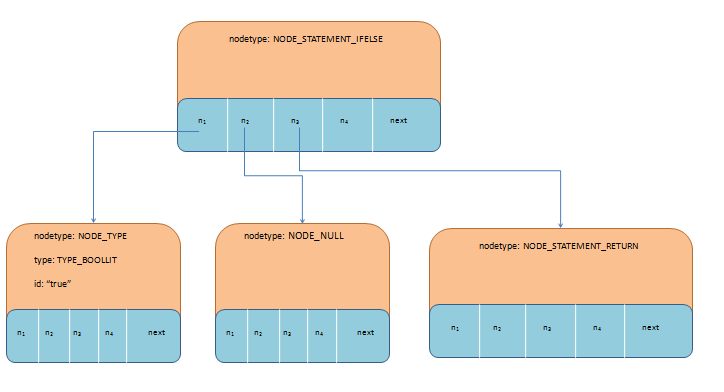
\includegraphics[width=\textwidth,height=\textheight,keepaspectratio]{If_Statement.png}
  \caption{Representação gráfica de um nó do tipo ``If''. No caso, representa a expressão \emph{if ( true ) {} else return;.}}
\end{figure}

A árvore e o nó estão intimamente relacionados.  De facto, uma árvore fica definida como o nó da sua raíz. Dado um dado nó, existe uma árvore com raíz nesse nó.

Os filhos $n_1$, $n_2$, $n_3$ e $n_4$ são utilizados para indicar nós filhos de um dado nó, nos casos em que se sabe que um dado nó terá um número fixo de filhos, e pela ordem em que surgem na gramática (esquerda, direita). Por exemplo, o nó $NODE\_STATEMENT\_ELSEIF$ tem, segundo a AST fornecida, de ter 3 nós. Desse modo, $n_1$, $n_2$ e $n_3$ estão preenchidos, respectivamente, com a condição, o statement correspondente à verificação da condição (``then'') e o statement correspondente à não verificação da condição (`else'').

Em anexo (Anexo A), apresentamos uma tabela que detalha a estruturação de todos os nós da AST. A regra ``geral'' a ter em conta é que sempre que um nó tem um potencial número variável de filhos, então armazena-os numa lista ligada, apontando para o primeiro nó da mesma, geralmente a partir de $n_1$, mas não necessariamente. Reiteramos que o Anexo A esclarece todas as dúvidas quanto à AST.

\begin{figure}[H]
  \centering
      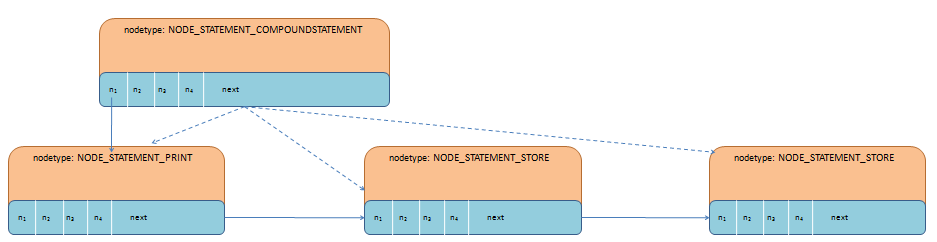
\includegraphics[width=\textwidth,height=\textheight,keepaspectratio]{Compound_Statement.png}
  \caption{Representação gráfica de um nó do tipo ``Compound Statement''. A tracejado encontra-se uma representação mais conceptual da árvore, enquanto que as setas preenchidas indicam a verdadeira representação interna da mesma.}
\end{figure}

\begin{figure}[H]
  \centering
      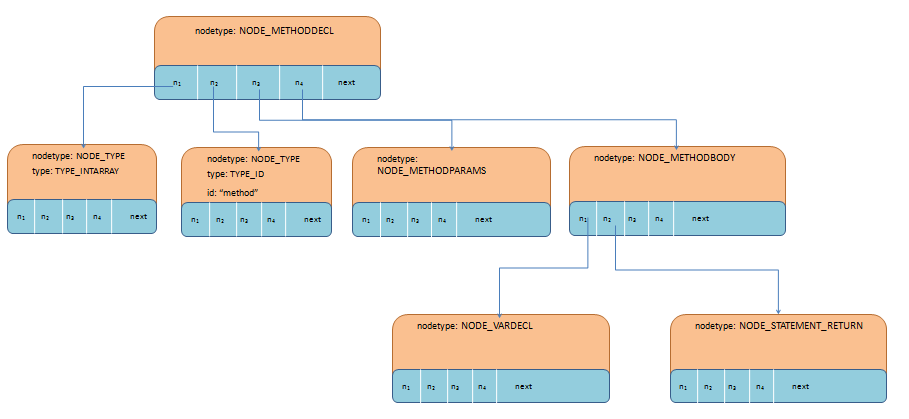
\includegraphics[width=\textwidth,height=\textheight,keepaspectratio]{Method_Decl.png}
  \caption{Representação gráfica de um nó do tipo ``MethodDeclaration''. Este é o único nó que utiliza todos os ponteiros ($n_1$, $n_2$, $n_3$, $n_4$ e, potencialmente, $next$).}
\end{figure}

\subsection{Construção da árvore}

\subsubsection{Métodos auxiliares}

A par da estrutura $node\_t$, existe ainda um conjunto de funções que auxiliam a manipular e criar nós. No espírito da programação orientada a objectos, existe uma função de criação de nós, $node\_create$, que apenas serve de base (é invocada por) outras funções, uma por cada nó que existe na AST. Assim, existem, por exemplo, $node\_create\_vardecl$, $node\_create\_methodbody$, etc. Em particular, no caso dos operadores binários e unários, recorremos a macros que geram estas funções e suas declarações por nós.

Para ligar nós uns aos outros (utilizando o next), implementámos o método $node\_append$, que adiciona a lista começada pelo segundo argumento ao final da lista começada pelo primeiro argumento.

\subsubsection{YACC}

Utilizando o sistema de pilha interno do $YACC$, fazendo uso das $unions$ descritas na análise lexical, criamos nós quando chegamos a uma folha e propagamo-los, subindo na árvore, utilizando o método $node\_append$ sempre que necessário. Deste modo, como temos um método individual para todos os nós, e uma só estrutura, bem como o sistema de pilha do $YACC$, o código torna-se limpo e fácil de implementar.

\subsubsection{CompoundStatements}

Os CompundStatements são um caso particular e que se desvia levemente do resto do código. Uma vez que temos um símbolo $Statements$, que permite construir listas de $Statements$, aproveitámos este facto para introduzir uma versão modificada do $node\_append$, que aceita argumentos nulos, o $node\_statement\_append\_statement$ (e que internamente utiliza o $node\_append$), Para além disso, quando encontramos a regra \emph{Statement: OBRACE Statements CBRACE}, invocamos a função   \\* $node\_create\_statement\_potential\_compoundstatement$, que, ou retorna a lista de statements que recebe (criada durante o processo de criação da árvore do $YACC$), ou então retorna um recém-criado nó do tipo   \\* $NODE\_STATEMENT\_COMPOUNDSTATEMENT$, cujo $n_1$ aponta para a lista passada (caso haja mais de 2 statements na lista). Esta função limita-se, pois, a agir diferenciadamente consoante o número de nós na lista que recebe.

\subsubsection{Nós null}

Conforme já referido, os nós null são explicitamente criados, com o tipo $NODE\_NULL$, facto que facilita a impressão

\subsubsection{Impressão da AST}

Uma vez que apenas temos um tipo de nós, $node\_t$, a impressão pode ser feita de forma recursiva. Ao estabelecermos uma tabela de strings que aceita como índices os valores inteiros correspondentes à enumeração que representa o tipo de cada nó, podemos imprimir facilmente a representação em string de cada nó. Por exemplo, para obter o nome do nó $x$, basta-nos aceder a $tabela[x->nodetype]$. Na verdade, recorremos a duas tabelas, já que o nó do tipo $NODE\_TYPE$ pode ter diferentes strings que lhe correspomde, e que são estas mapeadas de acordo com outra tabela para a enumeração $ijavatype\_t$.

A impressão é, pois, feita de forma recursiva, passando como argumento a profundidade, seguindo sempre os ponteiros $n\_1$, $n\_2$, $n\_3$ e $n\_4$, primeiramente (para descer na árvore) e $next$, em segundo lugar, para percorrer o mesmo nível da árvore, da esquerda para a direita.

Esta tabela de lookup e o certo ``polimorfismo'' da nossa estrutura de dados permite, então, uma maneira simples e eficiente de fazer a impressão.

\pagebreak

\section{Análise Semântica}

	Até esta fase da compilação, os passos executados, estruturas criadas, etc tinham como principal objetivo certificar que o programa, de facto, estava escrito na linguagem \emph{iJava} adotada.
	
	Na fase da \emph{Análise Semântica} pretendemos alargar esse estudo, procurando aferir se as instruções que constituem o programa possuem, de facto, algum significado em \emph{iJava}.
	
	Assim, nesta fase da compilação, a principal preocupação irá recair sobre as operações a realizar indicadas no programa, verificando a compatibilidade dos tipos de dados envolvidos nestas. Nesse sentido, necessitamos de criar uma estrutura que, de alguma forma, nos permita armazenar e consultar as variáveis (e os respetivos tipos) a que podemos aceder a partir de uma qualquer zona do programa.
	
	Para tal, foi necessário criar e implementar \emph{Tabelas de Símbolos}, que nos permitem aceder a essas mesmas informações. Desta forma podemos verificar os tipos dos dados envolvidos nas diversas operações que constituem o programa, detectando eventuais situações de incompatibilidade entre tipos, inválidas nos programas.

	\subsection{Tabelas de Símbolos}
	
	Uma \emph{Tabela de Símbolos} (ou um \emph{Ambiente}) é, como já referimos, uma estrutura de dados que mapeia identificadores com os seus tipos e localizações.
	
	Como a nossa linguagem apenas permite a execução de programas com uma única classe, que possui métodos e atributos estáticos e públicos, necessitamos de conhecer todos os métodos e atributos que compõem a classe, bem como as variáveis definidas em cada um dos métodos.
	
	Desta forma podemos facilmente detectar situações em que são invocados métodos não declarados na classe, ou em que são utilizados atributos não definidos na classe ou para o método no qual se pretende utilizar o atributo. 

	Por estas razões mantemos uma \emph{Tabela de Símbolos} para a classe na qual está contido o programa, sendo também mantida uma \emph{Tabela de Símbolos} para cada método definido para a classe.
	
	\subsubsection{Criação das Tabelas de Símbolos}
	
	Cada \emph{Tabela de Símbolos} é criada a partir da \emph{Árvore de Sintaxe Abstrata}, construída na etapa anterior da compilação.
	
	Assim, para a criação da \emph{Tabela de Símbolos} da classe do programa, percorremos os nós da \emph{Árvore de Sintaxe Abstrata} relativos às declarações de atributos e métodos, criando uma nova entrada na tabela (ou uma tabela inteiramente nova) para cada método ou atributo declarado, na qual se armazenam o nome do método ou atributo declarado.
	
	No caso da entrada corresponder a um atributo é também armazenado o tipo do atributo. Caso a entrada corresponda à declaração de um método é guardado uma referência para a \emph{Tabela de Símbolos} do método.
	
	Na criação da \emph{Tabela de Símbolos} de um método da classe percorremos os nós da \emph{Árvore de Sintaxe Abstrata} relativos às instruções que compõem o método, criando na sua \emph{Tabela de Símbolos} uma entrada onde armazenamos o seu nome, outra onde é armazenado o tipo de retorno, e uma entrada para cada argumento ou variável local declarada, contendo o respetivo tipo.
	
	\subsubsection{Implementação}
	
	
	
	Na listagem que se segue, apresentamos a estrutura de dados utilizada para representar e implementar cada \emph{Tabela de Símbolos} criada, à qual demos o nome de \emph{sym\_t}:
	
	\begin{lstlisting}
typedef struct _sym_t sym_t;	

struct _sym_t{
	ijava_table_type_t node_type;
	char* id;
	ijavatype_t type;
	int is_parameter;
	sym_t* next;
	sym_t* table_method;
	node_t* method_start;
};

typedef enum {
	CLASS_TABLE,
	METHOD_TABLE,
	VARIABLE,
	METHOD
} ijava_table_type_t;
	\end{lstlisting}
	
	
	
	Chamamos também a atenção do leitor para a definição do tipo \\* \emph{ijava\_table\_type\_t}, apresentado a par da estrutura \emph{sym\_t}.
	
	Lembramos ainda que os tipos \emph{ijavatype\_t} e \emph{node\_t} foram apresentados na definição das estruturas utilizadas na \emph{Árvore de Sintaxe Abstrata}.
	
	Passemos a detalhar um pouco mais a implementação apresentada.
	
	\begin{figure}[H]
  \centering
      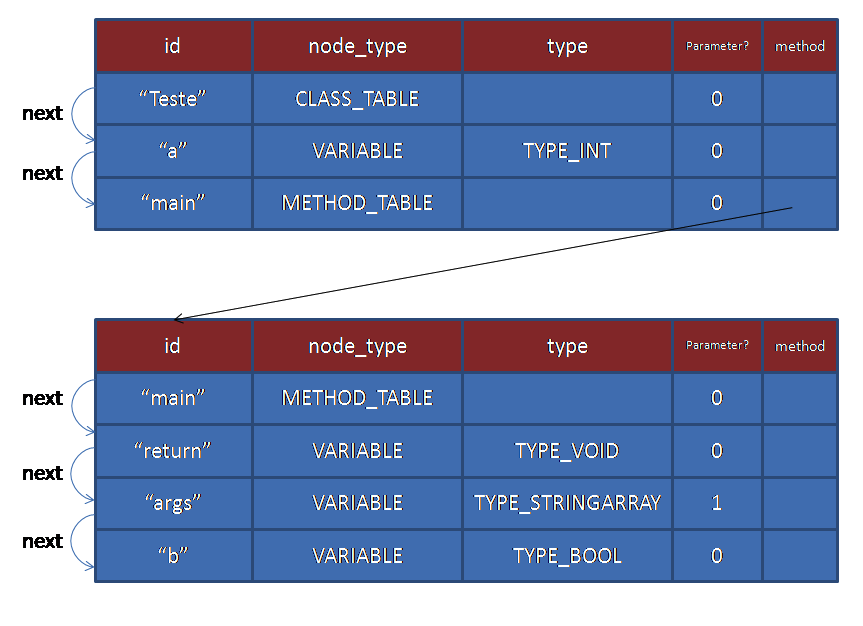
\includegraphics[width=\textwidth,height=\textheight,keepaspectratio]{Symbol_Table.png}
  \caption{Representação gráfica, conceptual, mas orientada para a implementação das tabelas de símbolos. As tabelas em si são listas ligadas, e cada entrada pode ser uma variável, uma entrada inicial com metadata, ou uma função (apontando para uma próxima tabela). Note-se que a primeira variável tem sempre o nome ``return'' e corresponde ao tipo de retorno de um método.}
\end{figure}
	
	Cada entrada da \emph{Tabela de Símbolos} corresponde a uma estrutura do tipo \emph{sym\_t}, sendo cada tabela constituída por uma ou mais entradas.
	
	As nossas \emph{Tabelas de Símbolos} não passam de simples listas ligadas, onde o primeiro elemento (a cabeça da lista) caracteriza a tabela, possuindo informação relativa ao seu nome (que coincide com o nome da classe ou do método em questão), armazenado em \emph{id}, e tipo, que se encontra em \emph{node\_type}. O tipo indica-nos se a entrada em questão corresponde a uma tabela de uma classe ou de um método, ou a uma declaração de um método ou de uma variável. Os diferentes elementos da lista encontram-se ligados pelo valor armazenado em \emph{next}, um ponteiro para o próximo elemento da lista.
	
	No caso da \emph{Tabela de Símbolos} da classe, os restantes elementos vão corresponder a declarações de atributos ou métodos, possuindo no seu campo \emph{id} o nome do atributo ou método declarado. Os que correspondem a declarações de atributos da classe vão possuir o seu tipo (\emph{int}, \emph{boolean}, etc) armazenado em \emph{type}. Já os que correspondem a declarações de métodos referenciam a \emph{Tabela de Símbolos} desse método através do campo  \emph{table\_method}. Adicionalmente, estes últimos possuem também no campo \emph{method\_start} uma referência para o nó da \emph{Árvore de Sintaxe Abstrata} onde se encontra a declaração do método.
	
	Relativamente à \emph{Tabela de Símbolos} de um método, o seu primeiro elemento está de acordo com o descrito anteriormente. Segue-se um elemento que contém o tipo de retorno do método, armazenado no campo \emph{type}. Posteriormente encontram-se os argumentos do método, no caso de existirem, também eles com a informação relativa ao nome e tipo presente em \emph{id} e \emph{type}, respetivamente. Estes elementos possuem também o valor $1$ no campo inteiro \emph{is\_parameter}, que indica que se tratam de parâmetros do método. Por fim, encontram-se as variáveis locais, pela ordem de declaração no método, sendo a informação relativa ao seu nome e tipo armazenada nos campos \emph{id} e \emph{type}, respetivamente.

	\subsubsection{Detecção de erros semânticos nas declarações}
	É durante a construção das tabelas de símbolos que também verificamos se existem declarações inadequadas (múltiplas, por exemplo). Se, por exemplo, tentarmos inserir duas vezes uma variável com um dado nome numa dada tabela, teremos encontrado uma definição múltipla.

	\subsubsection{Impressão}
	A impressão das tabelas de símbolos faz-se novamente com recurso a uma tabela de lookup, como já outrora feito para a AST. Este mecanismo permite-nos facilmente modificar todas as strings que esperamos que apareçam no ecrã aquando do output desta tabela.
	
	\subsubsection{Conclusão}
	
	Após a análise das estruturas de dados apresentadas podemos retirar algumas conclusões acerca das implicações que a escolha destas estruturas teve na implementação das \emph{Tabelas de Símbolos}.
	
	É clara a utilização da mesma representação para estruturas conceptualmente distintas, como é o caso da tabela de símbolos da classe e dos métodos, ou das declarações de atributos e métodos de uma classe.
	
	De facto, reconhecemos que a utilização de diferentes estruturas seria mais adequado de um ponto de vista conceptual, já que nos permitiria distinguir melhor os elementos que pretendemos representar, evitando a existência de campos não utilizados em algumas estruturas.
	
	No entanto, optámos por manter esta representação dado que a consideramos mais simples ao nível da implementação, permitindo-nos generalizar algumas operações como a impressão dos elementos das diferentes tabelas, e até a procura de um elemento numa tabela.
	
	\pagebreak
	
	\subsection{Detecção de Erros Semânticos (para além de declarações)}
	
	A detecção dos restantes erros semânticos faz-se percorrendo recursivamente a AST, tomando partido de algumas informações armazenadas na tabela de símbolos. A ideia geral do algoritmo consiste em iterar sobre todos os statements e avaliar a sua validade semântica. Para tal, aplicamos um algoritmo recursivo nas expressões que os envolvem. Por exemplo, no statement $System.out.println(a[2])$, percorreremos recursivamente o operando ``a[2]" (do tipo $LOADARRAY$) e os seus operandos (``a'' e ``2''). Expressões complexas são decompostas e analisadas recursivamente, verificando se estão a ser aplicadas a tipos correctos e se os tipos são coerentes entre si.
	
	No caso particular da maior parte dos operadores binários, possuímos inclusivamente o conjunto de macros que funcionam quase como ``regras'' da aplicação deste operador e que são quase auto-explicativas. Um excerto:
	
	\begin{lstlisting}
	  int is_binary_operator_allowed(nodetype_t oper, ijavatype_t lhstype, ijavatype_t rhstype) {
    ALLOW_BIN_OPER_SAMETYPE_BOOL(NODE_OPER_AND);
    ALLOW_BIN_OPER_SAMETYPE_BOOL(NODE_OPER_OR);

    ALLOW_BIN_OPER_SAMETYPE_ALL(NODE_OPER_EQ);	
    ALLOW_BIN_OPER_SAMETYPE_ALL(NODE_OPER_NEQ);
    
    ALLOW_BIN_OPER_SAMETYPE_INT(NODE_OPER_LT);
    ALLOW_BIN_OPER_SAMETYPE_INT(NODE_OPER_GT);
    ALLOW_BIN_OPER_SAMETYPE_INT(NODE_OPER_GEQ);
    ALLOW_BIN_OPER_SAMETYPE_INT(NODE_OPER_LEQ);
    ALLOW_BIN_OPER_SAMETYPE_INT(NODE_OPER_ADD);
    ALLOW_BIN_OPER_SAMETYPE_INT(NODE_OPER_SUB);
    ALLOW_BIN_OPER_SAMETYPE_INT(NODE_OPER_MUL);
    ALLOW_BIN_OPER_SAMETYPE_INT(NODE_OPER_DIV);
    ALLOW_BIN_OPER_SAMETYPE_INT(NODE_OPER_MOD);
   	 
   ALLOW_BIN_OPER(NODE_OPER_LOADARRAY, TYPE_INTARRAY, TYPE_INT);
   ALLOW_BIN_OPER(NODE_OPER_LOADARRAY, TYPE_BOOLARRAY, TYPE_INT);


    ALLOW_BIN_OPER(NODE_OPER_PARSEARGS, TYPE_STRINGARRAY, TYPE_INT);
             

	return 0;
}
	\end{lstlisting}
	
	Torna-se claro que este método é como que uma tabela de regras, o que facilita a implementação, a manutenção e, de certo modo, a portabilidade do código.
	
	No entanto, dados os constrangimentos de tempo do projecto, outros operadores e outros statements não foram implementados com o mesmo sistema, não invalidando a correcção dos mesmos.
	
	A função recursiva que progressivamente analisa sub-árvores, obtém os seus tipos e verifica se são aplicáveis no contexto de um dado operador, chama-se $get\_tree\_type$, apesar de admitirmos que um nome mais apropriado talvez fosse $get\_expression\_type$\footnote{A ideia do nome original advém do facto de estarmos a obter o ``tipo'' da subárvore passada como argumento}.
	
	A recursividade pára quando se alcança um nó do tipo $NODE_TYPE$, que tanto pode ter um tipo directamente associado (isto é, ser um literal, como ``true'' ou ``0xAB''), como referenciar um outro id, caso em que se torna necessário aceder à tabela de símbolos\footnote{Mais precisamente, acede às várias tabelas de símbolos: a do método actualmente a ser analisado e a da tabela de símbolos da classe} para saber que tipo lhe corresponde. A informação dos tipos é depois propagada para as funções chamantes. Torna-se também necessário referir que a operação de invocação de funções também é um dos casos base de fim de recursividade. 
	
	Neste processo de análise, é ainda verificada a validade dos literais\footnote{Se não são demasiado largos, e se representam correctamente números.}, quando são encontrados no fim da recursividade.
	
	Caso um operador não possa aplicar-se aos tipos que foram já obtidos das sub-árvores da AST, o programa termina com um erro semântico apropriado
	
	Relativamente ao método que percorre os statements, chama-se \\* $recurse\_down$, pois é responsável por iniciar o processo recursivo de análise de statements individuais. Para além disso, invoca-se a si mesmo, recursivamente, caso alcance um Compund Statement.
	
	Destacamos ainda que não percorremos de novo toda a AST para fazer esta análise. Em vez disso, durante o processo de construção das tabelas de símbolos, armazenamos ponteiros para os nós da AST que dizem respeito a cada função. Deste modo, apenas precisamos de percorrer todos os métodos que temos na tabela de símbolos e seguir os ponteiros deles para os nós respectivos da AST.
	
	\pagebreak
	
\section{Geração de Código}

A geração de código faz-se de uma forma extremamente semelhante à maneira como fazemos a análise sintáctica. Na verdade, ambas as tarefas podiam unir-se numa só, e optámos por não o fazer por questões de facilidade de implementação, modularização de código e constrangimentos de tempo.

De facto, a geração de código consiste em percorrer a AST e, para cada nó, produzir um conjunto de instruções correspondentes à representação intermédia $LLVM$ $IR$, que geralmente se mapeiam quase directamente. Por exemplo os operadores binários correspondem todos a uma única instrução simples, havendo mapeamento directo entre nós da árvore e instruções $LLVM$ $IR$.

A AST é percorrida exactamente da mesma forma que na análise semântica, gerando primeiro o código para obter os resultados de subexpressões. Por exemplo, em $(a+b)+c$, primeiro é gerado o código para obter o valor de $(a+b)$ numa variável temporária, que depois é passada à operação de soma em conjunto com $c$. Esta lógica recursiva é a que já antes encontrámos durante a análise semântica, com a diferença de que nesta última procurávamos obter os tipos de subexpressões (e, portanto subárvores), enquanto que na geração de código procuramos obter os resultados destas.

\subsection{Variáveis temporárias}

O nosso código faz uso extensivo de variáveis temporárias pertencentes a funções. Implementámos um método $get\_local\_var\_name$, que nos retorna a próxima variável temporária a utilizar. Sendo assim, retornará progressivamente $\%1$, $\%2$, $\%3$, etc. Este contador de variáveis é reinicializado sempre que entramos na geração de código para uma nova função. Optámos por abstrair este comportamento numa função, em vez de manualmente lidar com o contador de variáveis, para permitir que outros métodos de obter variáveis temporárias possam mais tarde vir a ser implementados -- trata-se de uma camada de abstracção adicional.

\subsection{Labels}
Ao longo do código precisaremos de utilizar labels, emparilhadas com statements de branching. Para tal, implementámos um contador que nunca reinicia e que constrói labels da forma ``label1'', ``label2'', etc. Não há, deste modo, qualquer informação ``útil'' de debugging nos nossos nomes de labels, escolha que tomámos por rapidez de implementação.

\subsection{Estruturas de dados}

Ao longo do nosso código de geração de $LLVM$ $IR$, a estrutura de dados mais utilizada é o tipo de dados $llvm\_var\_t$, que representa uma variável actualmente existente no código gerado. Ela associa informação sobre a sua representação (``$\%variavel$'', por exemplo), o tipo de dados associado ($TYPE\_INT$, por exemplo) e se a variável tem memória associada (globais e pilha) ou não. Esta última noção é internamente referida como ``ser value''. Consideramos que uma variável é um ``value'' se não tiver memória associada, isto é, se for temporária. Ao mantermos a informação sobre quais variáveis são temporárias ou não, ficamos a saber se temos de fazer loads, por exemplo. A declaração da estrutura que temos vindo a abordar é a seguinte:

\begin{lstlisting}
  typedef struct _llvm_var_t {
    char* repr; /* Representation: %1,@1, etc... */
    ijavatype_t type; /* TYPE_INTARRAY, TYPE_INT... */
    int value; /* Raw value or pointer? */
} llvm_var_t;
\end{lstlisting}

A par desta estrutura, existem métodos para a criar e destruir, bem como alguns métodos auxiliares. Por exemplo, existe um método que obtém uma variável não alocada (``temporária'' / ``loaded''\footnote{Ao longo do código, utilizamos também a ideia de uma variável estar ``loaded'' se tiver $value = 1$, isto é, não necessitar de um $load$ para os acessos aos dados.}) a partir de uma alocada.

\subsection{Retorno de métodos}

O ``return'' foi implementado recorrendo a uma label de retorno (uma por cada função) e uma variável alocada na pilha onde se guadarão os valores a retornar. A variável é declarada como ``.return'', para garantir que tal nome não existe em iJava. Deste modo, um return é equivalente ao ``pseudo-LLVM''\footnote{Utilizamos um híbrido entre LLVM e assembly, em que omitimos o type-checking, para facilitar a leitura.}:

\begin{lstlisting}
  store %retorno, %.return
  goto .return
\end{lstlisting}

A existência de uma label garante que o retorno por defeito é garantido aquando da alocação da variável de retorno na pilha (é o valor com que a inicializamos), e torna o fluxo do código fácil de analisar. Também nos permite escrever um só epílogo de função, em vez de ter de escrever vários antes de cada statement de return.

Por questões de facilidade de implementação, todos os métodos void retornam um inteiro na nossa implementação.

\subsection{Declaração de funções e armazenamento de parâmetros na pilha}
Para permitir a modificação de variáveis passadas como argumentos, torna-se necessário armazenar os parâmetros que são passados às funções na pilha. Para tal, optámos por os declarar com um ``.'' no início do nome, e o nome sem o ponto é utilizado para a variável alocada na pilha.

Por exemplo, a seguinte implementação em $iJava$:
\begin{lstlisting}
  public static void function(int a, int b, boolean c, int[] d) {}
\end{lstlisting}

produz o seguinte código (comentado e indentado a posteriori):
\begin{lstlisting}
define i32 @function(i32 %.a, i32 %.b, i1 %.c) {
  %return = alloca i32, align 4
  store i32 0, i32* %return             ; Inicializar a zero o valor de retorno
  %a = alloca i32, align 4               
  store i32 0, i32* %a                     
  store i32 %.a, i32* %a                  ; Guardar a na pilha
  %b = alloca i32, align 4
  store i32 0, i32* %b
  store i32 %.b, i32* %b                 ; Guardar b na pilha
  %c = alloca i1, align 4
  store i1 0, i1* %c    
  store i1 %.c, i1* %c                      ; Guardar c na pilha
\end{lstlisting}

Observamos também algumas redundâncias do nosso código, como inicializações a zero seguidas de substituições desses mesmos valores. Tal código é aceitável e válido.

\subsection{Arrays}

Os arrays foram implementados recorrendo a uma estrutura do LLVM em que armazenamos tanto o tamanho como um ponteiro para o array em si. Dado que suportamos dois tipos de arrays, temos duas destas estruturas, emitidas no preâmbulo do ficheiro de output:

\begin{lstlisting}
%.IntArray = type { i32, i32* }
%.BoolArray = type { i32, i1* }
\end{lstlisting}

Utilizando as instruções $getelementptr$, store e a keyword $null$, é-nos possível indexar e aceder aos vários arrays. Por uma questão de implementação (e debugging), os arrays são os únicos casos em que utilizamos variáveis temporárias com um nome mais explícito do que apenas um número. Mais concretamente, se um array se chamar $variavel$, geraremos as variáveis temporárias $.array.variavel$ e $..array.variavel$\footnote{A utilização dos pontos evita name clashing com o iJava, enquanto que a palavra ``array'' evita name-clashing interno com outras variáveis.}.

\subsection{Short-circuiting}

Tal como requerido pela linguagem iJava, torna-se necessário implementar short-circuiting, isto é, garantir que apenas avaliamos as expressões que temos necessariamente de avaliar. A nossa implementação reside no facto de o seguinte código

\begin{lstlisting}
a = b && c;
\end{lstlisting}

ser equivalente a

\begin{lstlisting}
a = b;
if ( a ) a = c;
\end{lstlisting}

ou, de outra forma (mais facilmente automatizável)

\begin{lstlisting}
tmp = b;
if ( tmp ) tmp = c;
a = tmp;
\end{lstlisting}

Algo semelhante pode ser conseguido para o operador OR, pois, de facto,

\begin{lstlisting}
a = b || c;
\end{lstlisting}

é equivalente a

\begin{lstlisting}
tmp = b;
if ( !tmp ) tmp = c;
a = tmp;
\end{lstlisting}

É desta forma que implementamos short-circuiting em iJava, recorrendo a uma variável temporária intermédia e utilizando ifs. 

Concretamente, e a título de exemplo, o seguinte excerto de código
\begin{lstlisting}
a = b && c;
\end{lstlisting}

produz (indentado e comentado):

\begin{lstlisting}
%1 = alloca i1, align 4   ; tmp
store i1 0, i1* %1           ; Inicializado a zero (escusado)
%2 = load i1* %b
store i1 %2, i1* %1         ; tmp = b
%3 = load i1* %1

; if ( tmp ) goto %label1; else goto %label2
br i1 %3, label %.label1, label %.label2  

.label1:
    %4 = load i1* %c
    store i1 %4, i1* %1     ; tmp = c
br label %.label2            ; goto %label2
.label2:
    %5 = load i1* %1                                   
    store i1 %5, i1* %a     ; c = tmp
\end{lstlisting}

Novamente, neste excerto observam-se pequenas ineficiências no nosso código, como inicializações a zero de variáveis que não precisavam de ser assim inicializadas.

\subsection{Prólogo e epílogo}

A implementação de uma função, no nosso compilador, possui duas estapas à parte, que consistem na emissão do prólogo e do epílogo.

No prólogo:

\begin{itemize}
  \item Colocam-se os parâmetros na pilha
  \item Aloca-se espaço para a variável de retorno
\end{itemize}

No epílogo:

\begin{itemize}
  \item Coloca-se o retorno da função
\end{itemize}

Optámos por fazer esta divisão conceptual porque se relaciona com a implementação mais baixo-nível de código deste género.

\subsection{Operador new}

O operador new foi implementado internamente recorrendo ao calloc. Escolhemos o calloc e não o malloc porque este inicializa a zero, um pré-requisito do iJava. Este operador cria um novo array com o tamanho e a memória dada e coloca-o numa variável, podendo este ser depois atribuído a outra variável. A título de exemplo, o seguinte excerto de código (assume-se que $a$ é global):

\begin{lstlisting}
  a = new int[100];
\end{lstlisting}

produz (indentado e comentado)

\begin{lstlisting}
  %1 = add i32 0, 100
; Alocar o novo array
%2 = alloca %.IntArray, align 8
    ; (Iniciar a Zero)
    %.array.2 = getelementptr inbounds %.IntArray* %2, i32 0, i32 0
    store i32 0, i32* %.array.2, align 4
    %..array.2 = getelementptr inbounds %.IntArray* %2, i32 0, i32 1
    store i32* null, i32** %..array.2, align 8

;Armazenar tamanho
%3 = getelementptr inbounds %.IntArray* %2, i32 0, i32 0
store i32 %1, i32* %3, align 4

;Alocar bloco com calloc
%4 = call noalias i8* @calloc(i32 %1, i32 4) nounwind
%5 = bitcast i8* %4 to i32* 
%6 = getelementptr inbounds %.IntArray* %2, i32 0, i32 1

;Guardar bloco no array
store i32* %5, i32** %6, align 8

;Copiar array para o array a
%7 = load %.IntArray* %2
store %.IntArray %7, %.IntArray* @a
\end{lstlisting}

Realçamos o facto de a última etapa deste código ser gerada aquando do processamento do operador de atribuição (statement $STORE$).

No caso de variáveis globais, utilizamos o $zeroinitializer$ para garantir inicialização a zero de todos os campos de uma estrutura definida em $LLVM$ $IR$. Por exemplo:

\begin{lstlisting}
  @a = global %.IntArray zeroinitializer, align 8
\end{lstlisting}

\subsection{Statements if-else e while}

Os statements condicionais e de repetição são implementados recorrendo a labels de maneira bastante autoexplicativa. Podemos reparar que

\begin{lstlisting}
  if ( A ) { B } else { C }
\end{lstlisting}

é equivalente a

\begin{lstlisting}
  if ( A ) goto thenlabel; else goto elselabel;
  thenlabel:
    B;
    goto endifelselabel;
  elselabel;
    C
  goto endifelselabel;
\end{lstlisting}

Tal facto permite-nos gerar uma representação intermédia que mapeia quase perfeitamente para esta generalização do if. Se concretizarmos com um pseudo-exemplo:

\begin{lstlisting}
  if ( A ) { B } else { C }
\end{lstlisting}

produzirá

\begin{lstlisting}
  %1 = load i1* @A
br i1 %1, label %.label1, label %.label2
.label1:
... B ...
br label %.label3
.label2:
... C ...
br label %.label3
.label3:
\end{lstlisting}

Conforme esperávamos pela nossa simplificação do if em instruções mais pequenas. O mesmo podemos fazer para o while.

De facto,

\begin{lstlisting}
  while ( A ) { B }
\end{lstlisting}

é equivalente a

\begin{lstlisting}
  labeltest:
    if ( A ) goto labelcontinue; else goto labelendwhile;
  labelcontinue;
    B
  goto labeltest;
\end{lstlisting}

E, de facto, o anterior ``pseudo-código'' produz:

\begin{lstlisting}
br label %.label1
.label1:                  ;labeltest
%1 = load i1* @A

;if ( A ) goto labelcontinue; else goto labelendwhile;
br i1 %1, label %.label2, label %.label3
.label2:                  ;labelcontinue
... B ... 
br label %.label1 ; goto labeltest;
.label3:             ; labelendwhile
\end{lstlisting}

\subsection{Acesso a parâmetros da linha de comandos}
Para aceder aos parâmetros da linha de comandos, temos de lidar com a representação interna do $LLVM$ $IR$ destes parâmetros, que é em tudo similar à do C, com um $argc$ e um $argv$. Por forma a facilitar a nossa implementação, o nosso código renomeia todas as referências à variável do pseudo-tipo $StringArray$ para .args, um nome que sabemos que não entra em conflito com nenhum outro. Também por questões de implementação, o parâmetro $argc$ chamar-se-á $.args.length$.



\subsubsection{Operador .length}
O caso particular do operador .length para $StringArray$ é gerido simplesmente acedendo o parâmetro $.args.length$, depois de este ter sido decrementado por uma unidade (para excluir o nome do programa da contagem de argumentos).

\subsubsection{Integer.parseInt}

O operador $Integer.parseInt$ é em si implementado percorrendo o array de strings que o $LLVM$ nos fornecem tendo o cuidado de somar um offset de um para evitar aceder ao nome do programa.

O seguinte exomplo demonstra o acesso a parâmetros da linha de comandos:

\begin{lstlisting}
public static void function(String[] args) {
        int c;
        c = args.length;

        c = Integer.parseInt(args[2]);
    }
\end{lstlisting}

produzindo (indentado e comentado):

\begin{lstlisting}
define i32 @function(i32 %args.length, i8** %args) {
    ;Retorno
    %return = alloca i32, align 4
    store i32 0, i32* %return

    ;Local
    %c = alloca i32, align 4
    store i32 0, i32* %c

    ;Subtrair ao .length
    %1 = sub i32 %args.length, 1

    ;Armazenar em %c
    store i32 %1, i32* %c

    ; Indice
    %2 = add i32 0, 2

    ; Offset a somar
    %3 = add i32 %2, 1

    ; Aceder ao parametro
    %4= getelementptr inbounds i8** %args, i32 %3
    %5 = load i8** %4
    %6 = call i32 @atoi(i8* %5) nounwind readonly

    ;Armazenar
    store i32 %6, i32* %c

    ;Epilogo
    br label %.return1
    .return1:
    %.return_final = load i32* %return
    ret i32 %.return_final
}
\end{lstlisting}

\subsection{Impressão no ecrã}

Imprimir no ecrã é conseguido invocando a função printf com uma de três strings. Caso se trate de um inteiro, é-he passada a string ``%s\n'' e como segundo argumento o valor de do inteiro a imprimir. Caso se trata de um booleano, é efectuada uma conversão rápida com uma lookup table que transforma o booleano $0$ ou $1$ num ponteiro para ``false\n'' ou ``true\n'', respectivamente.

Esta tabela e estas strings são emitidas no preâmbulo:

\begin{lstlisting}

; String 'false\n'
@str.false_str = private unnamed_addr constant [7 x i8] c"false\0A\00"

; String 'true\n'
@str.true_str = private unnamed_addr constant [7 x i8] c"true\0A\00\00"

; Lookup table que mapeia as strings
@str.bools_array = global [2 x i8*] [i8* getelementptr inbounds ([7 x i8]* @str.false_str, i32 0, i32 0), i8* getelementptr inbounds ([7 x i8]* @str.true_str, i32 0, i32 0)]
\end{lstlisting}

\subsection{Operações aritméticas unárias}

A implementação de operações unárias foi simples, pois todas podem ser convertidas em operações binárias. De facto, apesar de até podermos evitar o unário ``+'', optámos por o reduzir a uma operação binária na mesma. Estas reduções são dadas pelas seguintes igualdades:

$$
-a = 0 - a
$$
$$
+a = 0 + a
$$
$$
!a = a\;\; xor\;\; true
$$

Com estas igualdades podemos, então, reduzir uma expressão unária a uma expressão binária.

\subsection{Comparações booleanas}

As operações booleanas são implementadas recorrendo ao operador $icmp$ e aos seus parâmetros, dados pela tabela seguinte:

\pagebreak

\begin{table}
    \begin{tabular}{ll}
    Operação      & Equivalente (para icmp) \\
    $=$             & eq                      \\
    $\neq$ & neq                     \\
    $<$             & slt                     \\
    $>$             & sgt                     \\
    $\leq$ & sle                     \\
        $\geq$ & slg                     \\
    \end{tabular}
\end{table}

Por exemplo, o seguinte código

\begin{lstlisting}
  a = 5 <= 2;
\end{lstlisting}

produz

\begin{lstlisting}
%2 = add i32 0, 5
%3 = add i32 0, 2
%4 = icmp sle i32 %2, %3
store i1 %4, i1* %1
%5 = load i1* %1
store i1 %5, i1* %a
  
\end{lstlisting}

\subsection{Restantes operações e statements}

A implementação das restantes operações e statements é intuitiva e auto-explicativa. Praticamente todos os operadores têm equivalentes em $LLVM$ facilmente mapeáveis e a simples leitura do código é suficiente para compreender.

\pagebreak

\section{Apreciação do Trabalho}

Fomos capazes de desenvolver um compilador para a linguagem apresentada no tempo disponível. Utilizámos boas técnicas de programação (uso frequente de $assert$s) para nos auxiliar neste processo. Tomámos várias decisões arquitecturais que moldaram o nosso programa, como a escolha de ter um nó único, um tipo único para a tabela de símbolos, tabelas de lookup, um único return, etc. Estas escolham provaram ser eficientes e práticas, uma vez que o nosso código está suficientemente faseado para podermos retirar os incrementos que adicionámos, mostando boas abstracções e práticas de engenharia de software que ``descolam'' os componentes uns dos outros.

No processo, desenvolvemos sistemas internos de teste e aprofundámos os nossos conhecimentos sobre o $yacc$, o $flex$\footnote{Ao longo deste relatório não elaborámos quanto ao funcionamento interno destes analisadores por considerarmos que tal está fora do âmbito do projecto, mas foi no contexto desse mesmo que nos familiarizámos com estes.} e sobre formas de representar árvores de sintaxe abstractas, tabelas de símbolos e processos de geração de código. Ambientámo-nos ao $LLVM$, tendo uma aproximação ligeira de geração de código. Produzimos um compilador funcional, com boas abstracções e relativamente fácil de modificar (para adição de futuras funcionalidades).

Achamos, por isso, que não voltaríamos atrás nas decisões de desenvolvimento que tivemos. De facto, durante o próprio projecto foram várias as vezes em que demos um passo atrás, anulando certas decisões (como, por exemplo, uma decisão inicial de não usar prioridades para tornar a gramática não ambígua). Estamos satisfeitos com o resultado do nosso trabalho, com a certeza de que num projecto com mais tempo estruturaríamos melhor certas partes do código e seríamos capazes de produzir compiladores para outras linguagens, inclusivamente linguagens que lidem com outros conceitos, como o de orientação a objectos e polimorfismo.

\end{document}